\documentclass[journal,10pt,twocolumn]{article}
\usepackage{graphicx, float}
\usepackage[margin=0.5in]{geometry}
\usepackage{amsmath, bm}
\usepackage{array}
\usepackage{booktabs}
\usepackage[utf8]{inputenc}
\usepackage{amsfonts}
\usepackage{amssymb}
\usepackage{graphicx}
\usepackage{multicol}
\usepackage{tabularx}
\usepackage{hyperref}
\DeclareUnicodeCharacter{2212}{-}
\providecommand{\norm}[1]{\left\lVert#1\right\rVert}
\providecommand{\sbrak}[1]{\ensuremath{{}\left[#1\right]}}
\providecommand{\lsbrak}[1]{\ensuremath{{}\left[#1\right.}}
\providecommand{\rsbrak}[1]{\ensuremath{{}\left.#1\right]}}
\providecommand{\brak}[1]{\ensuremath{\left(#1\right)}}
\providecommand{\lbrak}[1]{\ensuremath{\left(#1\right.}}
\providecommand{\rbrak}[1]{\ensuremath{\left.#1\right)}}
\providecommand{\cbrak}[1]{\ensuremath{\left\{#1\right\}}}
\providecommand{\lcbrak}[1]{\ensuremath{\left\{#1\right.}}
\providecommand{\rcbrak}[1]{\ensuremath{\left.#1\right\}}}
\newcommand{\myvec}[1]{\ensuremath{\begin{pmatrix}#1\end{pmatrix}}}
\let\vec\mathbf

\title{\textbf{Circle Assignment}}
\author{Namrath Pinnamaneni \hspace{9cm} FWC22042}
\date{September 2022}

\begin{document}

\maketitle
\paragraph{\textit{Problem Statement} - Find equation of the circle which touches the line \(2x + 3y + 1\) at the point (1, −1) and cuts orthogonal the circle which has the line segment joining (0, 3) and (−2, −1) as a diameter.}

\section*{\large Solution}

\begin{figure}[H]
\centering
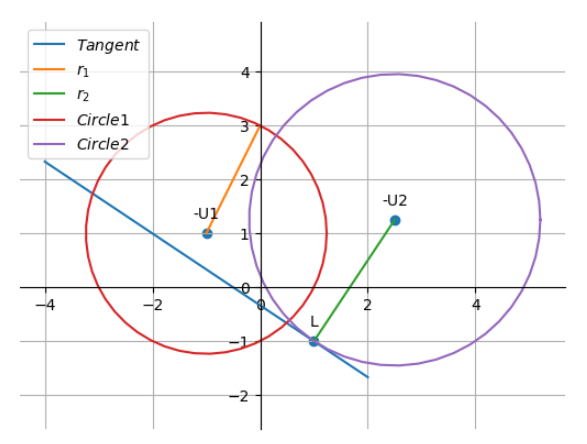
\includegraphics[width=1\columnwidth]{circles.png}
\caption{Tangents from A to circle through B, C and D}
\label{fig:triangle}
\end{figure}

With the given end vertices A(0,3) and B(-2,-1), we can find out centre \(U_1\) and radius \(r_1\) of Circle-1. We know that tangent \(2x+3y+1=0\) touches Circle-2 at L(1,-1) hence using mentioned we will solve for centre and radius of Circle-2 i.e.   \(U_2\) and \(r_2\) using 3 equations as follows. \vspace{4mm}

\textbf{STEP-1}\vspace{3mm}\\
Calculating $\vec{U_1}$ using  $\vec{A}\myvec{0\\3}$ and $\vec{B}\myvec{-2\\-1}$ \vspace{2mm}
\begin{equation}
\vec{U_1} = \frac{\vec{A}+\vec{B}}2
\end{equation}\vspace{1mm}\\ 
Centre of Circle-1, $\vec{U_1}$ = $\myvec{-1 \\ 1}$\vspace{2mm}\\ 
Calculating $r_1$ using $\vec{A}\myvec{0\\3}$ and $\vec{U_1}\myvec{-1\\1}$ \vspace{1mm}
\begin{align}
r_1 &= \norm{\vec{U_1} - \vec{A}} 
\end{align}
Radius of Circle-1, $r_1$ = $\sqrt{5}$\vspace{3mm}\\
\textbf{STEP-2}\vspace{2mm}\\
As both the circles are orthogonal, we get: \\\vspace{1mm}
\begin{align}
\norm{\vec{U_2} - \vec{U_1}}^2 = r_1^2 + r_2^2
\end{align}
\begin{align}
    \implies \norm{\vec{U_2}}^2 + \norm{\vec{U_1}}^2 - 2\vec{U_1}^{\top}\vec{U_2} = r_1^2 + r_2^2
\end{align}
Equation when tangent touches a Circle at a point L
		    \begin{align}
			    \vec{m}^{\top} \brak{\vec{L}+\vec{U_2}} = 0 \\
			    \implies \vec{m}^{\top}\vec{U_2} = - \vec{m}^{\top}\vec{L} 
		    \end{align}
We get $\vec{m}$ by
\begin{align}
\vec{m} = \vec{I}\vec{n}
\end{align}

\begin{center}
where $\vec{I} = \myvec{0 & -1 \\ 1 & 0}$, $\vec{n} = \myvec{2 \\ 3}$ \\
\end{center}
Finally we also know that,
\begin{align}
\norm{\vec{L} - \vec{(-U_2)}}^2 = r_2^2
\end{align}
\begin{align}
    \implies \norm{\vec{L}}^2 + \norm{\vec{U_2}}^2 + 2\vec{L}^{\top}\vec{U_2} = r_2^2
\end{align}    

\textbf{STEP-3}\vspace{2mm}\\   
After substituting \textbf{(9)} in \textbf{(4)} we get,
\begin{align}
2\brak{\vec{L}+\vec{U_1}}^{\top}\vec{U_2} = \norm{\vec{U_1}}^2 - \norm{\vec{L}}^2 - r_1^2
\end{align}

By using \textbf{(6)} and \textbf{(10)},

\begin{center}
$ 2\brak{\vec{L}+\vec{U_1}}^{\top}\vec{U_2} = \norm{\vec{U_1}}^2 - \norm{\vec{L}}^2 - r_1^2 $ \\
\end{center}

\begin{center}
$ \vec{m}^{\top}\vec{U_2} = - \vec{m}^{\top}\vec{L} $ \\
\end{center}
 
yielding, 
\begin{align}
\implies \myvec{2\brak{\vec{L}+\vec{U_1}}^{\top} \\ \vec{m}^{\top}}\vec{U_2} = \myvec{\norm{\vec{U_1}}^2 - \norm{\vec{L}}^2 - r_1^2 \\ \vec{m}^{\top}\vec{L}} 
\end{align}
solving we get, 
\begin{align}
\vec{U_2} = \myvec{2.5 \\ 1.25}
\end{align}
therefore we get r2,
\begin{align}
r_2 = \norm{\vec{U_2} - \vec{L}}
\end{align}
\begin{center}
    $r_2$ = 2.704
\end{center}

\section*{\large Construction}
{
\setlength\extrarowheight{5pt}
\begin{tabular}{|c|c|c|}
	\hline
	\textbf{Symbol}&\textbf{Value}&\textbf{Description}\\
	\hline
	$\vec{A,B}$&$\myvec{0 \\ 3},\myvec{-2 \\ -1}$&Given diametric points of $U_1$\\
	\hline
	$\vec{U_1}$&$\myvec{-1 \\ 1}$&Centre of Circle $U_1$\\
	\hline
	$r_1$ & $\sqrt{5}$ & Radius of Circle $U_1$\\
	\hline
	$\vec{L}$&$\myvec{1 \\ -1}$&Point at which Tangent touches $U_2$\\
	\hline
	$\vec{m}$&$\myvec{-3 \\ 2}$&Direction vector of Tangent\\
	\hline
	$\vec{U_2}$&$\myvec{2.5 \\ 1.25}$&Centre of Circle $U_2$\\	
	\hline
	$r_2$ & 2.704 & Radius of Circle $U_2$\\
	\hline
\end{tabular}
}

\end{document}